\documentclass[11pt]{article}
\usepackage[margin=1in]{geometry}
\usepackage{amsmath,amssymb}
\usepackage{booktabs}
\usepackage{hyperref}
\usepackage{url}
\usepackage{graphicx}
\usepackage{listings}
\usepackage{xcolor}

\lstset{
  basicstyle=\ttfamily\small,
  breaklines=true,
  frame=single,
  backgroundcolor=\color{gray!10}
}

\title{Supplementary Materials\\[0.5em]
\large Evaluating Tool-Using Language Agents: Judge Reliability,
Propagation Cascades, and Runtime Mitigation in AgentProp-Bench}
\date{}

\begin{document}
\maketitle

\tableofcontents
\newpage

% ============================================================================
\section{Code and Data Availability}

All code, data, and agent traces are publicly available at:
\url{https://github.com/bhaskargurram-ai/agenthallu-bench}

\noindent (Repository previously published as AgentHallu-Bench; see CHANGELOG.md.)

The repository contains:
\begin{itemize}
    \item \texttt{data/results/} --- Result CSVs and analysis JSONs
    \item \texttt{data/tasks/} --- 2,000 benchmark task specifications
    \item \texttt{experiments/} --- Experiment runner scripts
    \item \texttt{analysis/} --- Statistical analysis scripts
    \item \texttt{metrics/} --- EPS scorer and cascade detector
    \item \texttt{agent/} --- ReAct agent, model router, tool executor
    \item \texttt{benchmark/} --- Task generator and 4 domain API simulators
    \item \texttt{interceptor/} --- Runtime interceptor implementation
    \item \texttt{tests/} --- Unit tests
\end{itemize}

% ============================================================================
\section{Interceptor Threshold Sweep}

Table~\ref{tab:sweep} reports the full 12-configuration sweep on the
validation split ($n{=}40$ P2 rows, 2 models $\times$ 2 conditions
$\times$ 10 tasks).

% Source: analysis/interceptor_tuned_thresholds.json
\begin{table}[t]
\centering
\caption{Full interceptor threshold sweep. Each row is a configuration of the three-layer filter: L1 (tool-call repetition threshold), L2 (keyword match count), L3 (LLM self-check). Best configuration by $F_1$ is highlighted. $N = 960$ P2 sessions.}
\label{tab:sweep}
\begin{tabular}{r r c r r r r}
\toprule
L1 thresh & L2 kw & L3 & $F_1$ & Precision & Recall & Abstain\% \\
\midrule
1 & 2 & \checkmark & 0.842 $\star$ & 0.923 & 0.774 & 65.0 \\
1 & 2 & --- & 0.809 & 0.826 & 0.792 & 57.5 \\
1 & 3 & \checkmark & 0.808 & 0.955 & 0.700 & 55.0 \\
1 & 3 & --- & 0.776 & 0.826 & 0.731 & 57.5 \\
2 & 2 & \checkmark & 0.762 & 0.842 & 0.696 & 47.5 \\
2 & 2 & --- & 0.780 & 0.889 & 0.696 & 45.0 \\
2 & 3 & \checkmark & 0.810 & 0.850 & 0.773 & 50.0 \\
2 & 3 & --- & 0.833 & 0.938 & 0.750 & 40.0 \\
3 & 2 & \checkmark & 0.769 & 0.938 & 0.652 & 40.0 \\
3 & 2 & --- & 0.750 & 0.857 & 0.667 & 35.0 \\
3 & 3 & \checkmark & 0.667 & 0.824 & 0.560 & 42.5 \\
3 & 3 & --- & 0.800 & 0.933 & 0.700 & 37.5 \\
\bottomrule
\end{tabular}
\end{table}

% ============================================================================
\section{Self-Consistency Baseline ($k{=}3$)}

Table~\ref{tab:sc} reports per-model, per-condition results for $k{=}3$
self-consistency voting on 30 tasks per condition.
This section is directional only: at $n{=}30$ the comparison is
underpowered.

% Source: data/results/self_consistency_results.csv
\begin{table}[t]
\centering
\caption{Self-consistency analysis ($k = 3$ runs per task). Unique answers is the median count of distinct answers across repetitions. Hallucination rate is measured by heuristic match. Conditions: baseline (no injection) vs.\ P2 (semantic-wrong injection).}
\label{tab:selfconsistency}
\begin{tabular}{l l r r r r}
\toprule
Model & Condition & $n$ & Halluc.\% & Median uniq.\ ans. & Abstain\% \\
\midrule
DeepSeek-V3 & baseline & 30 & 30.0 & 2.0 & 46.7 \\
DeepSeek-V3 & p2_semantic & 30 & 23.3 & 3.0 & 60.0 \\
\midrule
GPT-4o-mini & baseline & 30 & 20.0 & 3.0 & 70.0 \\
GPT-4o-mini & p2_semantic & 30 & 23.3 & 3.0 & 56.7 \\
\bottomrule
\end{tabular}
\end{table}

% ============================================================================
\section{Cross-Domain Replication: Retail}

Table~\ref{tab:retail} reports baseline correctness and mean EPS on the
300 held-out retail tasks for three representative models.

% Source: data/results/baseline_retail.csv, data/results/p2_retail.csv
\begin{table}[t]
\centering
\caption{Cross-domain transfer: held-out retail tasks. Models were not exposed to retail tasks during P2 tuning. Correctness judged by heuristic match. 95\% bootstrap CIs ($B = 1{,}000$).}
\label{tab:retail}
\begin{tabular}{l r r l r r l}
\toprule
Model & $n_{\mathrm{BL}}$ & BL\% & CI & $n_{\mathrm{P2}}$ & P2\% & CI \\
\midrule
DeepSeek-V3 & 100 & 37.0 & [27.0, 47.0] & 100 & 43.0 & [33.0, 53.0] \\
GPT-4o-mini & 100 & 29.0 & [20.0, 38.0] & 100 & 33.0 & [24.0, 42.0] \\
Gemini-2.0-Flash & 100 & 17.0 & [10.0, 25.0] & 100 & 17.0 & [10.0, 25.0] \\
\bottomrule
\end{tabular}
\end{table}

% ============================================================================
\section{Interceptor Layer Ablation}

Table~\ref{tab:ablation} reports the ablation of interceptor layers on
GPT-4o-mini.

% Source: data/results/ablation_results.csv
\begin{table}[t]
\centering
\caption{Interceptor ablation study. Each condition removes one layer of the three-layer interceptor. Hallucination rate and abstain rate are reported. 95\% bootstrap CIs ($B = 1{,}000$).}
\label{tab:ablation}
\begin{tabular}{l l r r r r}
\toprule
Model & Condition & $n$ & Halluc.\% & Abstain\% & Correct\% \\
\midrule
Gemini-2.0-Flash & l1_l2 & 60 & 51.7 & 0.0 & 48.3 \\
Gemini-2.0-Flash & l1_l2_l3 & 60 & 48.3 & 1.7 & 50.0 \\
Gemini-2.0-Flash & l1_only & 60 & 48.3 & 0.0 & 51.7 \\
\midrule
GPT-4o-mini & l1_l2 & 60 & 46.7 & 11.7 & 41.7 \\
GPT-4o-mini & l1_l2_l3 & 60 & 41.7 & 26.7 & 31.7 \\
GPT-4o-mini & l1_only & 60 & 51.7 & 18.3 & 30.0 \\
\bottomrule
\end{tabular}
\end{table}

% ============================================================================
\section{Power Analysis}

Table~\ref{tab:power} reports Cohen's $h$ and achieved power for each
statistical claim in the paper.

% Source: recomputed from baseline_all.csv, p2_all_rejudged.csv, interceptor CSVs
\begin{table}[t]
\centering
\caption{Post-hoc power analysis for all main contrasts. Effect size is Cohen's $h$; achieved power is computed at $\alpha = 0.05$ (two-sided). Contrasts with power $< 0.80$ are flagged (\dag).}
\label{tab:power}
\small
\begin{tabular}{l r r r r r r}
\toprule
Contrast & $n_1$ & $n_2$ & $p_1$ & $p_2$ & $h$ & Power \\
\midrule
DeepSeek-V3: P2 vs BL & 450 & 200 & 0.482 & 0.625 & 0.288 & 0.924 \\
GPT-3.5-Turbo: P2 vs BL & 450 & 200 & 0.496 & 0.675 & 0.366 & 0.991 \\
GPT-4.1-mini: P2 vs BL & 450 & 200 & 0.453 & 0.655 & 0.409 & 0.998 \\
GPT-4.1-nano: P2 vs BL & 450 & 200 & 0.547 & 0.845 & 0.668 & 1.000 \\
GPT-4o-mini: P2 vs BL & 450 & 200 & 0.600 & 0.710 & 0.232 & 0.780$^{\dag}$ \\
Gemini-2.0-Flash: P2 vs BL & 450 & 200 & 0.524 & 0.670 & 0.298 & 0.939 \\
Qwen2.5-14B: P2 vs BL & 450 & 200 & 0.444 & 0.625 & 0.364 & 0.990 \\
Qwen2.5-3B: P2 vs BL & 450 & 200 & 0.458 & 0.825 & 0.792 & 1.000 \\
Qwen2.5-7B: P2 vs BL & 450 & 200 & 0.509 & 0.715 & 0.427 & 0.999 \\
o3-mini: P2 vs BL & 50 & 50 & 0.600 & 0.700 & 0.210 & 0.182$^{\dag}$ \\
GPT-4o-mini: Interceptor & 600 & 600 & 0.558 & 0.328 & -0.467 & 1.000 \\
Gemini-2.0-Flash: Interceptor & 600 & 600 & 0.445 & 0.432 & -0.027 & 0.068$^{\dag}$ \\
\bottomrule
\end{tabular}
\end{table}

% ============================================================================
\section{Per-Domain Propagation Rates}

Figure~\ref{fig:domain} shows per-domain stage-reach rates under P2
semantic-wrong injection.

\begin{figure}[h]
  \centering
  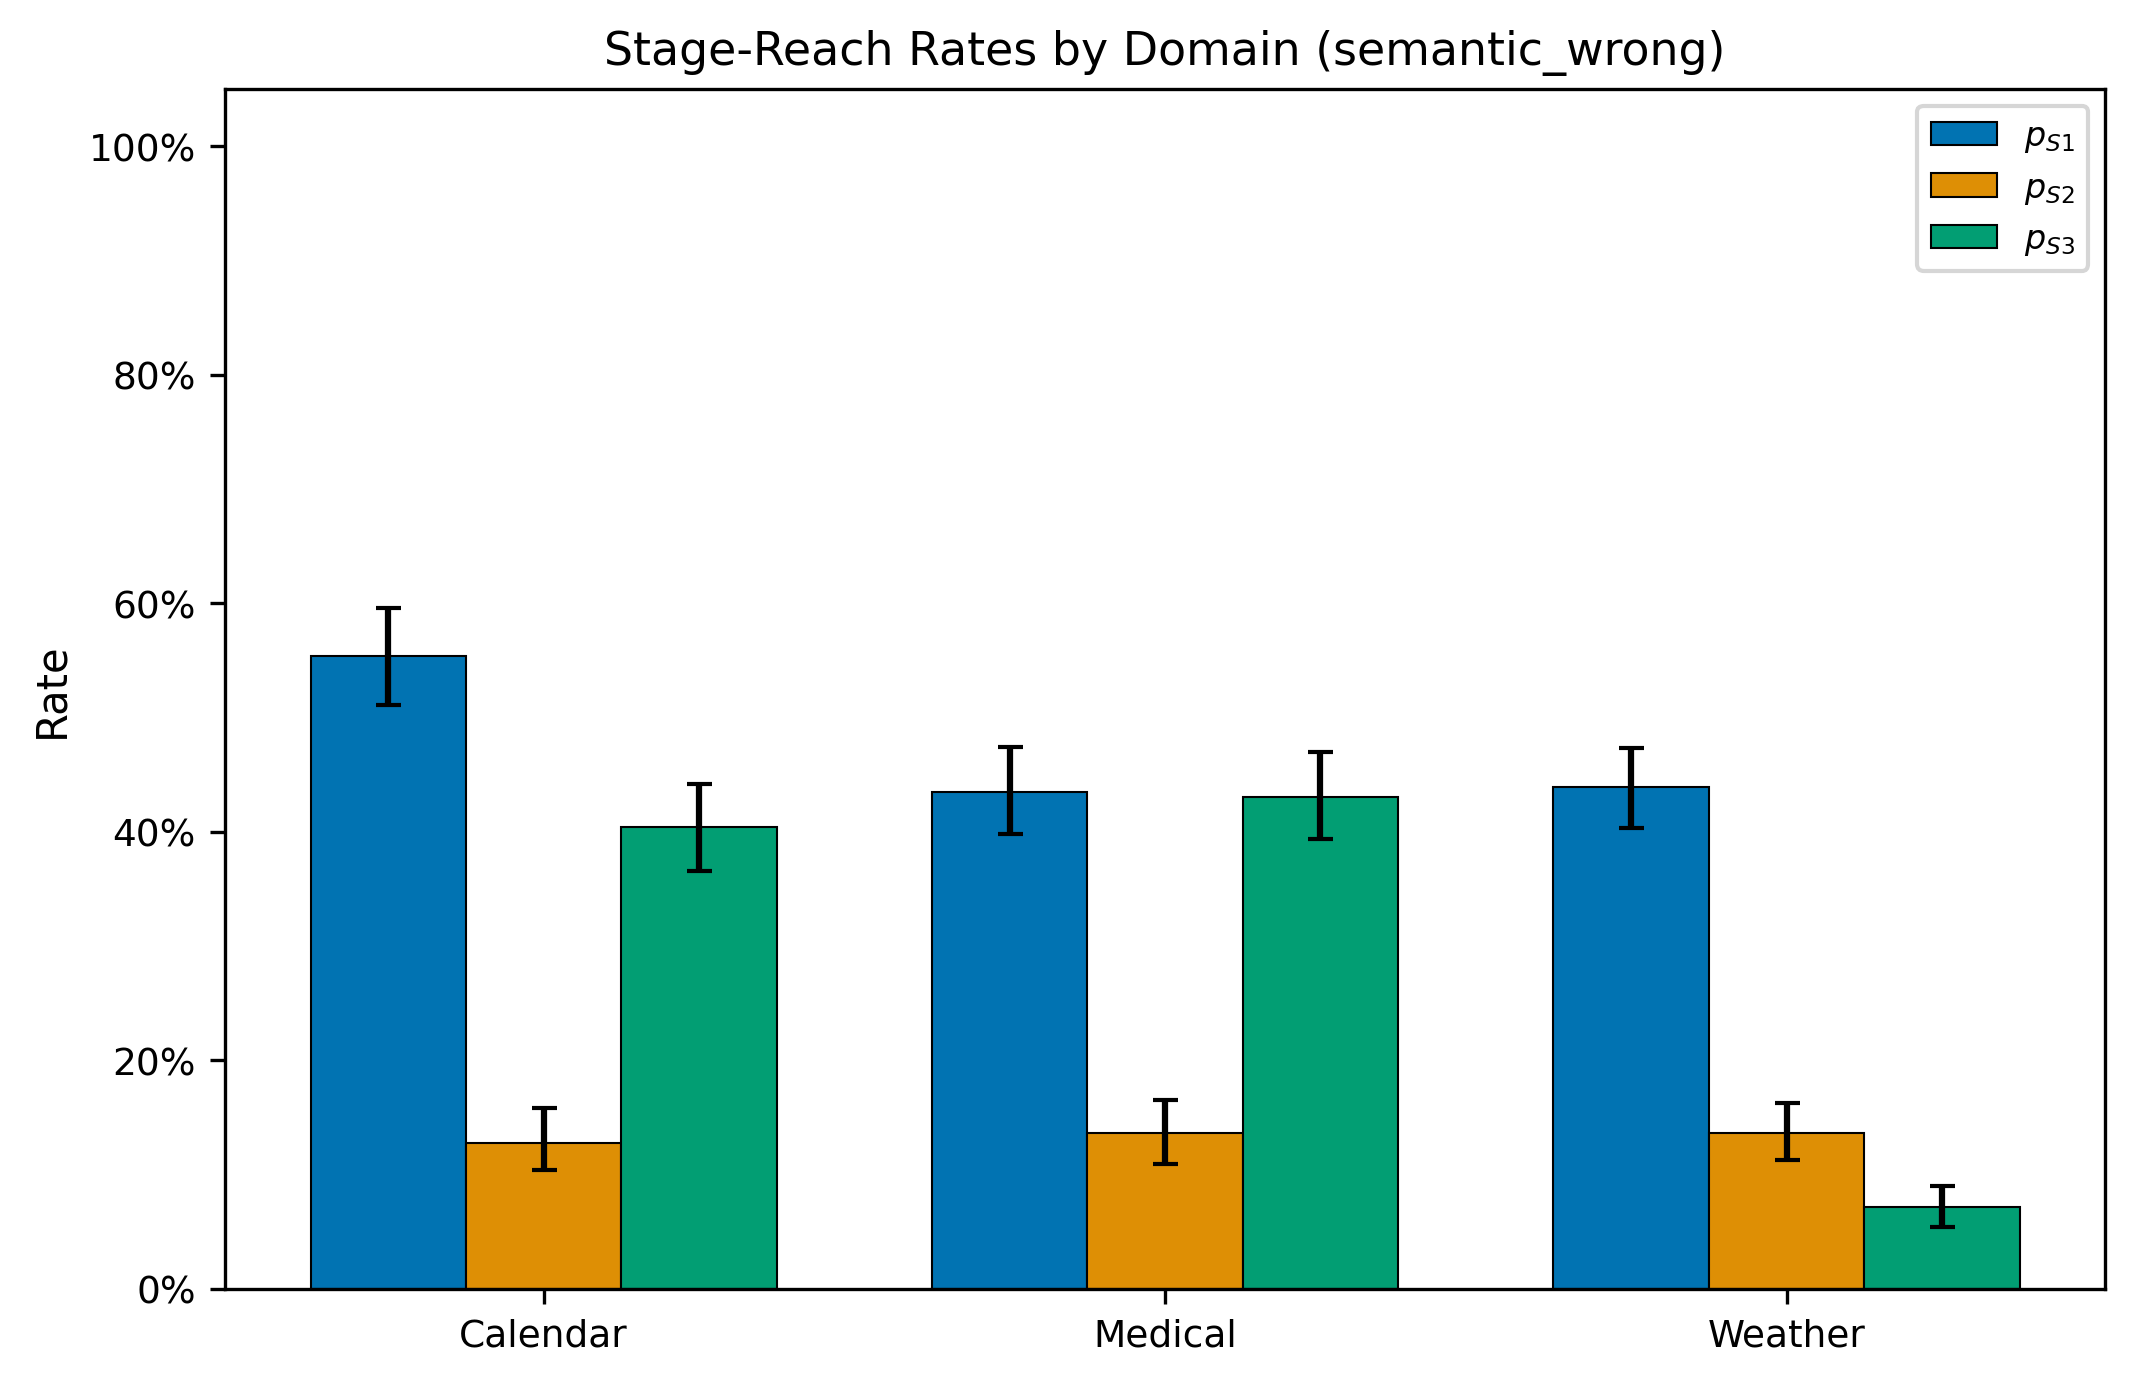
\includegraphics[width=0.8\textwidth]{figures/fig_domain_breakdown.png}
  \caption{Per-domain $S_1$, $S_2$, $S_3$ rates under P2 semantic-wrong
    injection (ensemble-judged). Calendar and weather domains show higher
    injection application rates than medical.}
  \label{fig:domain}
\end{figure}

% ============================================================================
\section{Human-Calibration Procedure}

Figure~\ref{fig:cal} visualizes the calibration relationship between
ensemble verdicts and human labels.

\begin{figure}[h]
  \centering
  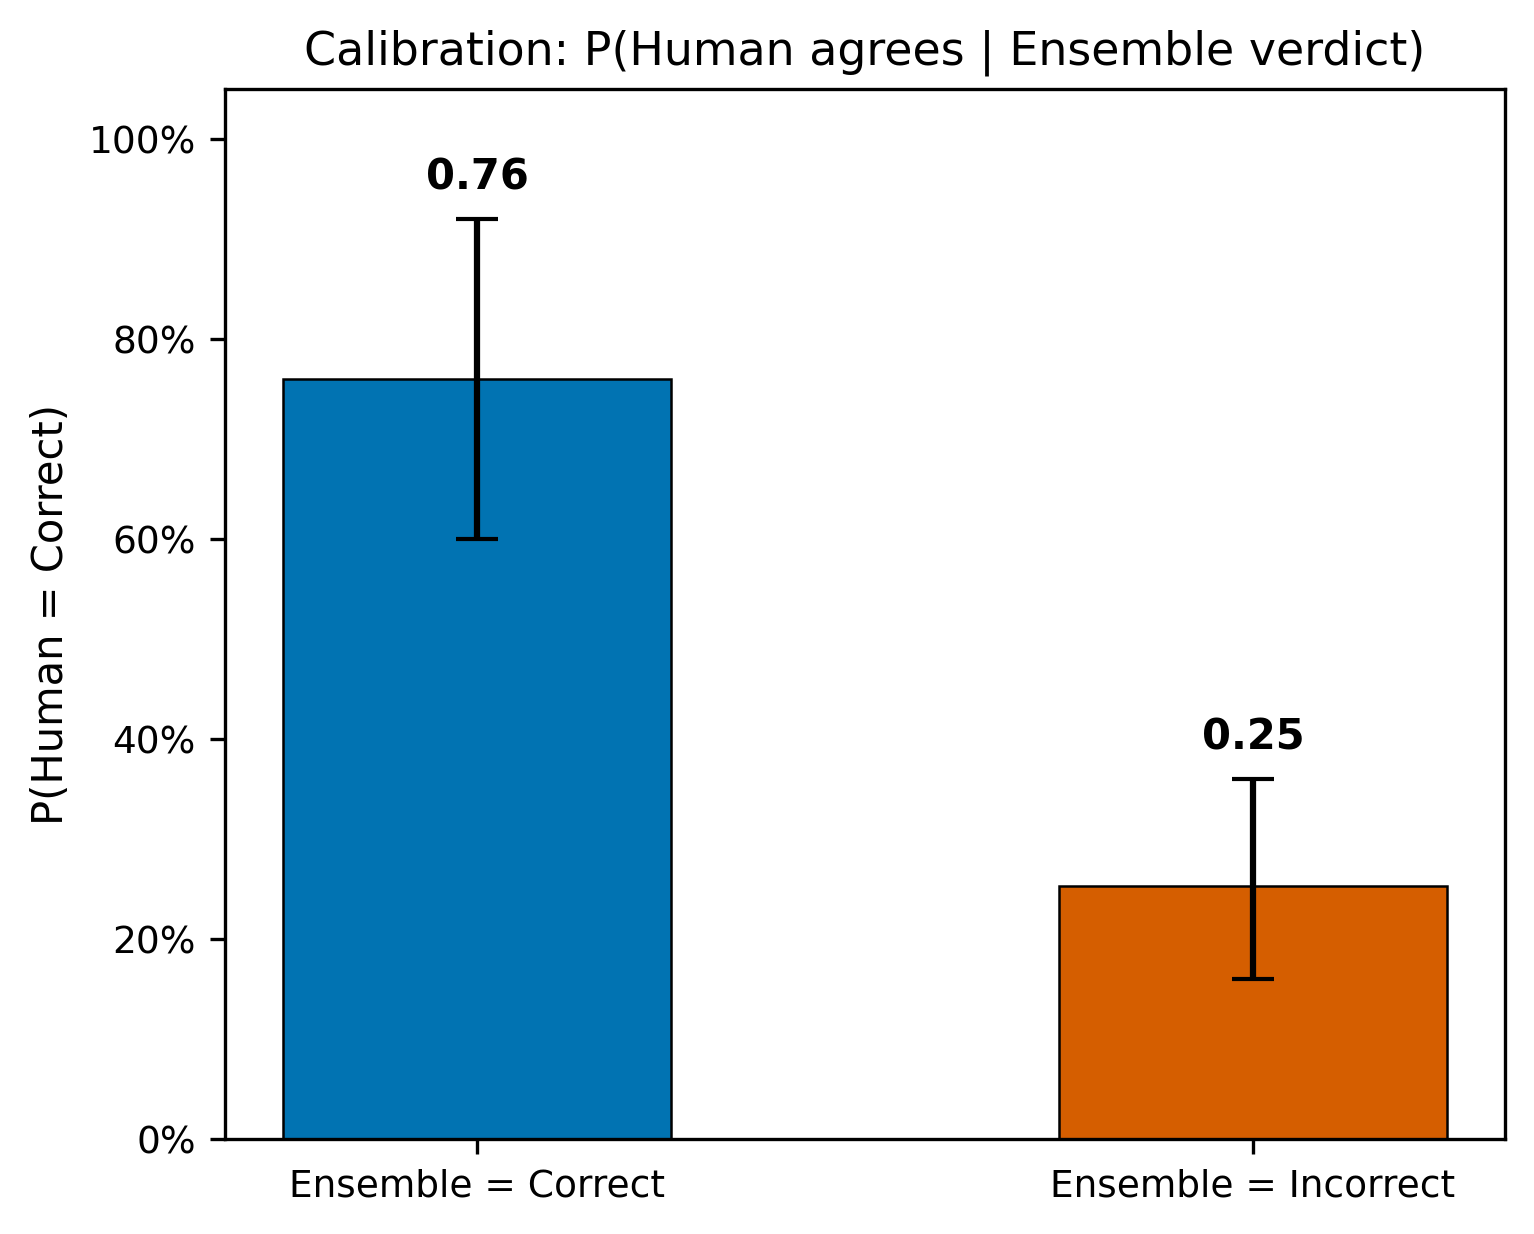
\includegraphics[width=0.6\textwidth]{figures/fig_calibration.png}
  \caption{Calibration of ensemble judge against 100 human labels.
    $P(\text{human=correct} \mid \text{ensemble=correct}) = 0.76$;
    $P(\text{human=correct} \mid \text{ensemble=wrong}) = 0.25$.
    The ensemble has a conservative bias (underreports correctness).}
  \label{fig:cal}
\end{figure}

% ============================================================================
\section{Ensemble Judge Prompt}

The following prompt is used identically for all three LLM judges
(GPT-4o, Gemini-2.5-Flash, GPT-4o-mini):

\begin{lstlisting}
You are an impartial judge evaluating whether an agent's
final answer is correct.

QUESTION: {query}
REFERENCE ANSWER: {reference}
AGENT ANSWER: {candidate}

Respond with a single token: YES if the agent answer
substantively matches the reference, NO otherwise.
Accept minor wording differences, units expressed
differently, or extra explanation as long as the core
fact is correct.

YOUR VERDICT (YES or NO):
\end{lstlisting}

% ============================================================================
\section{Confusion Matrix: Ensemble vs Human}

\begin{figure}[h]
  \centering
  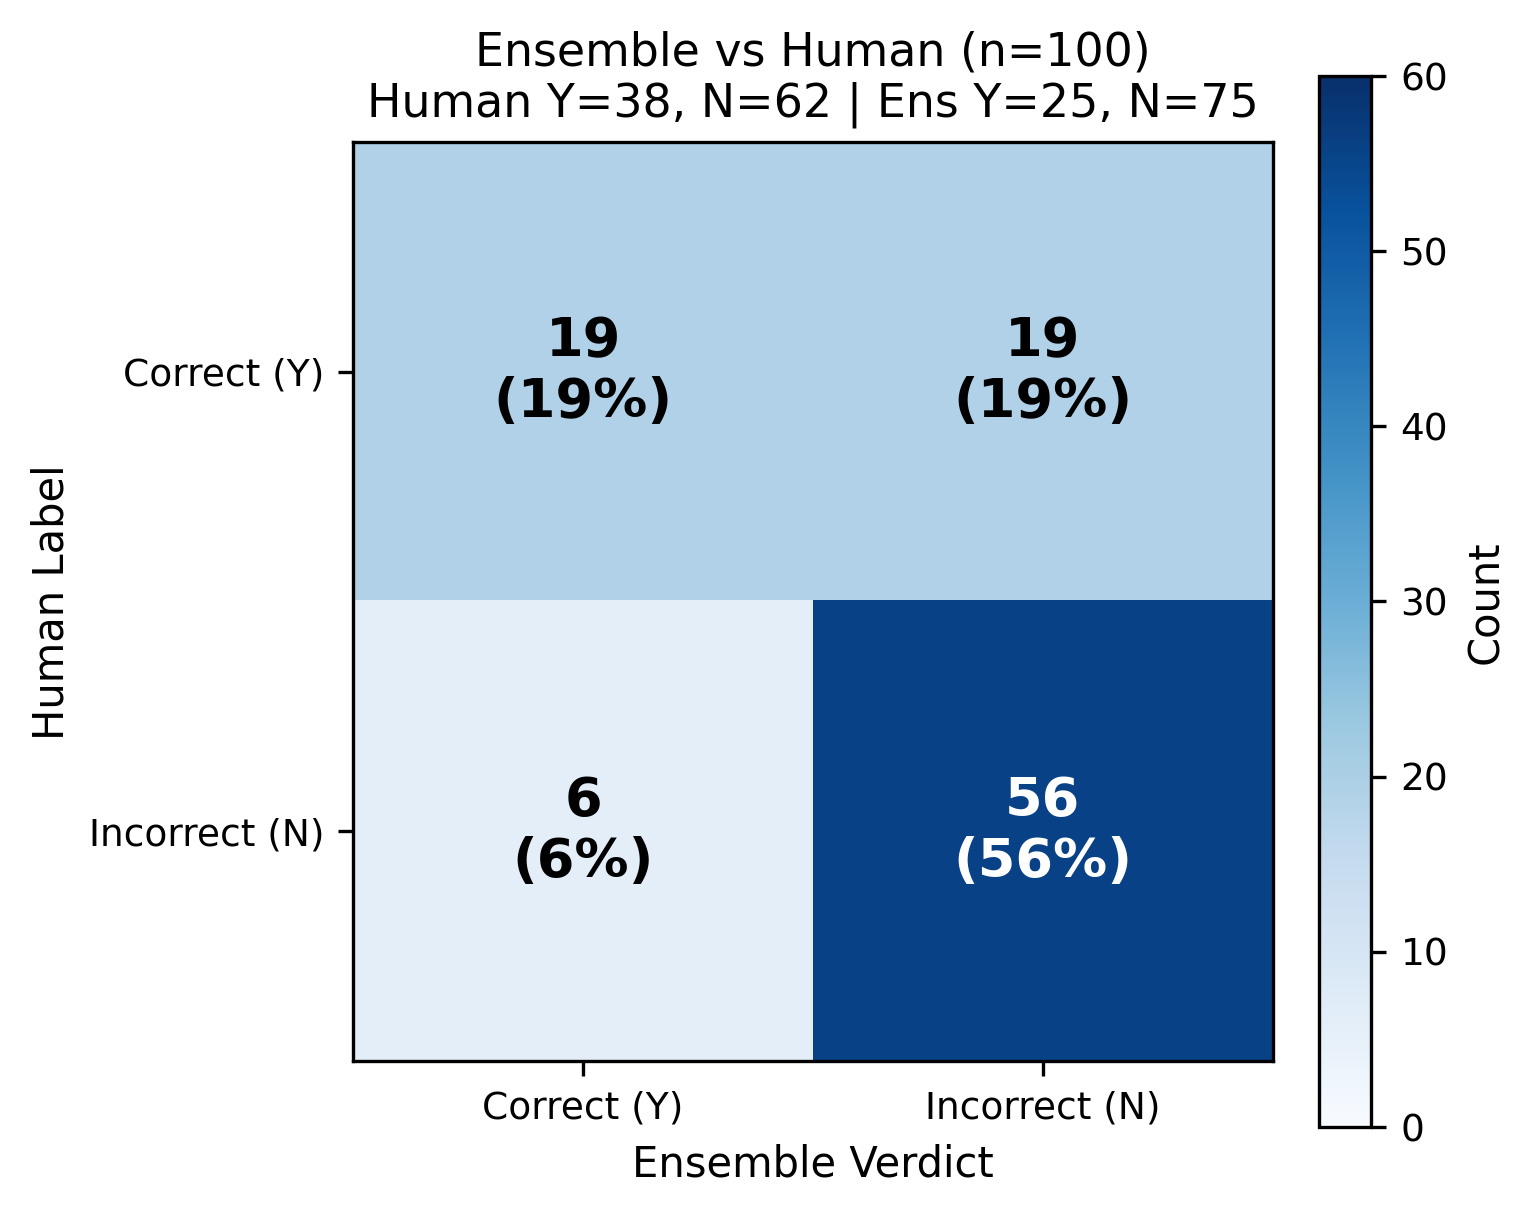
\includegraphics[width=0.5\textwidth]{figures/fig_confusion_matrix.png}
  \caption{Confusion matrix: ensemble judge vs.\ 100 human labels.
    The dominant disagreement is the ensemble rejecting answers that
    humans accept (19 traces).}
  \label{fig:confusion}
\end{figure}

% ============================================================================
\section{Dataset Statistics}

\begin{table}[h]
\centering
\caption{Dataset statistics by domain and split.}
\begin{tabular}{lrrrl}
\toprule
Domain & Tasks & Baseline traces & P2 traces & Role \\
\midrule
Calendar & 667 & 450 & 800 & Training/evaluation \\
Weather & 674 & 450 & 800 & Training/evaluation \\
Medical & 559 & 450 & 800 & Training/evaluation \\
Retail & 300 & 300 & 300 & Held-out replication \\
Knowledge & 100 & 100 & --- & Ablation only \\
\midrule
\textbf{Total} & \textbf{2,300} & \textbf{1,750} & \textbf{2,700} & \\
\bottomrule
\end{tabular}
\end{table}

\end{document}
